\documentclass[paper=a4, fontsize=11pt]{scrartcl} % A4 paper and 11pt font size
\usepackage[noend]{algpseudocode}
\usepackage{ctex}
\usepackage[utf8]{inputenc}
\usepackage{graphicx}

% Default fixed font does not support bold face
\DeclareFixedFont{\ttb}{T1}{txtt}{bx}{n}{12} % for bold
\DeclareFixedFont{\ttm}{T1}{txtt}{m}{n}{12}  % for normal

% Custom colors
\usepackage{color}
\definecolor{deepblue}{rgb}{0,0,0.5}
\definecolor{deepred}{rgb}{0.6,0,0}
\definecolor{deepgreen}{rgb}{0,0.5,0}
\usepackage{indentfirst}
\usepackage[T1]{fontenc} % Use 8-bit encoding that has 256 glyphs
\usepackage{fourier} % Use the Adobe Utopia font for the document - comment this line to return to the LaTeX default
\usepackage[english]{babel} % English language/hyphenation
\usepackage{amsmath,amsfonts,amsthm} % Math packages
\usepackage{listings}
\usepackage[english]{babel}
\usepackage[utf8]{inputenc}
\usepackage{algorithm}
\usepackage{lipsum} % Used for inserting dummy 'Lorem ipsum' text into the template

\usepackage{sectsty} % Allows customizing section commands
\allsectionsfont{\centering \normalfont\scshape} % Make all sections centered, the default font and small caps

\usepackage{fancyhdr} % Custom headers and footers
\pagestyle{fancyplain} % Makes all pages in the document conform to the custom headers and footers
\fancyhead{} % No page header - if you want one, create it in the same way as the footers below
\fancyfoot[L]{\normalfont Shanghai Jiao Tong University} % Empty left footer
\fancyfoot[C]{\thepage} % Empty center footer
\fancyfoot[R]{} % Page numbering for right footer
\renewcommand{\headrulewidth}{0pt} % Remove header underlines
\renewcommand{\footrulewidth}{0pt} % Remove footer underlines
\setlength{\headheight}{13.6pt} % Customize the height of the header

\numberwithin{equation}{section} % Number equations within sections (i.e. 1.1, 1.2, 2.1, 2.2 instead of 1, 2, 3, 4)
\numberwithin{figure}{section} % Number figures within sections (i.e. 1.1, 1.2, 2.1, 2.2 instead of 1, 2, 3, 4)
\numberwithin{table}{section} % Number tables within sections (i.e. 1.1, 1.2, 2.1, 2.2 instead of 1, 2, 3, 4)

\setlength\parindent{1pt} % Removes all indentation from paragraphs - comment this line for an assignment with lots of text
\usepackage{xcolor} % for setting colors
\usepackage{listings}

% Python style for highlighting
\newcommand\pythonstyle{\lstset{
language=Python,
basicstyle=\ttm,
otherkeywords={self},             % Add keywords here
keywordstyle=\ttb\color{deepblue},
emph={MyClass,__init__},          % Custom highlighting
emphstyle=\ttb\color{deepred},    % Custom highlighting style
stringstyle=\color{deepgreen},
frame=tb,                         % Any extra options here
showstringspaces=false            % 
}}
% Python for external files
\newcommand\pythonexternal[2][]{{
\pythonstyle
\lstinputlisting[#1]{#2}}}
% set the default code style

\renewcommand{\algorithmicrequire}{\textbf{Input:}}
\renewcommand{\algorithmicensure}{\textbf{Output:}}
\newcommand{\horrule}[1]{\rule{\linewidth}{#1}} % Create horizontal rule command with 1 argument of height
\title{	
\normalfont \normalsize 
\textsc{Probability Theory and Mathematical Statistics} \\ [25pt] % Your university, school and/or department name(s)
\horrule{1pt} \\[0.5cm] % Thin top horizontal rule
\huge \kaishu 利用蒙特卡洛估算积分 \\ % The assignment title
\horrule{2pt} \\[0.5cm] % Thick bottom horizontal rule
}
\newlength\myindent
\setlength\myindent{2em}
\newcommand\bindent{%
  \begingroup
  \setlength{\itemindent}{\myindent}
  \addtolength{\algorithmicindent}{\myindent}
}
\newcommand\eindent{\endgroup}
\author{\kaishu 吕艺\\ \normalsize 517021910745} % Your name

\date{\normalsize\today} % Today's date or a custom date

\begin{document}

\maketitle % Print the title
\section{\kaishu 适用范围}
在概率论与数理统计中,我们常常使用数学期望来描述随机变量的数字特征,其中涉及到函数在区间上的积分。在高等数学中,我们通常采用寻找原函数的方法来计算积分值,然而在实际生活中,很多随机变量的分布函数都是超越函数,不存在原函数,故寻找原函数这一方法失效。
当随机变量维度较低时,可以采用数值插入的方法。可当随机变量维度较高时,数值插入的方法就显得力不从心。此时通过蒙特卡洛方法,我们可以将问题转换为随机取样求平均值,从而进行积分的近似计算。
\section{\kaishu 数学原理}
假设我们有一个函数$k(x)$,当$k(x)$满足$k(x) \ge 0 , a \leq x \leq b$,且$\int _a^b k(x) = C <\infty$,则我们可以定义k(x)对应的概率密度函数
\begin{equation}
p(x) = \frac{k(x)}{C}
\end{equation}

根据这一原理,我们可以将复杂的分布函数转换为较为简单的分布函数。由于计算机的内部算法实现,大多计算机内部只能生成满足均匀分布或者高斯分布的随机数,这一转换对于利用计算机进行随机模拟有着很大的帮助。
\vspace{2cm}


利用类似思想,假设我们要计算的积分为$\int_a^b g(x) = I$,我们可将g(x)分解为$h(x)$和$p(x)$(其中$p(x)$通常为较为简单的概率密度函数,以方便取样模拟)。之后我们取一组相互独立,且在区间[a,b]上满足$p(x)$分布的随机变量$X_{i}$,那么$h(X_{i})$也为独立同分布的随机变量。
\begin{equation}	
E(h(X_{i})) = \int_a^b{h(X_{i}) \dot p(x)} =\int_a^b{g(X_{i})} = C
\end{equation}
则根据Khintchine定理,$X_{i}$满足大数定律,
\begin{equation}
	\lim_{N to \infty} P(| \dfrac{1}{N} \sum_{i=1}^{N} h(X_{i}) - \dfrac{1}{N}\sum_{i = 1}^{n}E(X_{i})|<\epsilon)=1
\end{equation}
因此,当N充分大的时候我们可以近似认为:
\begin{equation}
	\dfrac{1}{N} \sum_{i=1}^{N} h(X_{i}) \approx \dfrac{1}{N}\sum_{i = 1}^{n}E(X_{i})
\end{equation}
\begin{equation}
	C \approx \dfrac{1}{N} \sum_{i=1}^{N} h(X_{i})
\end{equation}

% 假设我们需要计算的积分为$I = \int_a^b k(x) dx$,由于a和b的取值范围不同,我们可以将近似估计的积分为定积分或广义积分两类。
\vspace{1cm}

\section{具体实现}
设待求积分为$\int_a^b{g(x)}$,根据a,b取值的不同,我们可以将模拟近似估计积分分为以下两种情况,分别为定积分和无穷积分。

1)定积分计算:   $\int_0^1{x e^{x}}$

首先通过分部积分确定该积分的值为1,之后利用MCMC方法模拟结果进行比较。由于在计算机中\emph{\textbf{定区间均匀分布}}的随机数比较容易获得,这里将g(x)拆分为:
\begin{gather*}
h(x) = x e^{x}  \qquad p(x) = 1
\end{gather*}

之后通过生成一满足服从(0,1)上均匀分布的随机序列,并将它们通过h(x)进行映射后的结果取平均值,从而得出随机模拟的估计值。

估算结果如下图所示。通过观察,在随机序列中的元素个数小于$10^{3}$时,MCMC估算误差较大,当随机序列个数大于$10^{3}$时,MCMC估算较为精确。由此可见,MCMC方法适用于估算定区间上的积分,且元素个数越大,MCMC的估计值与积分的实际值更接近。


\begin{figure}[H]
	\centering
	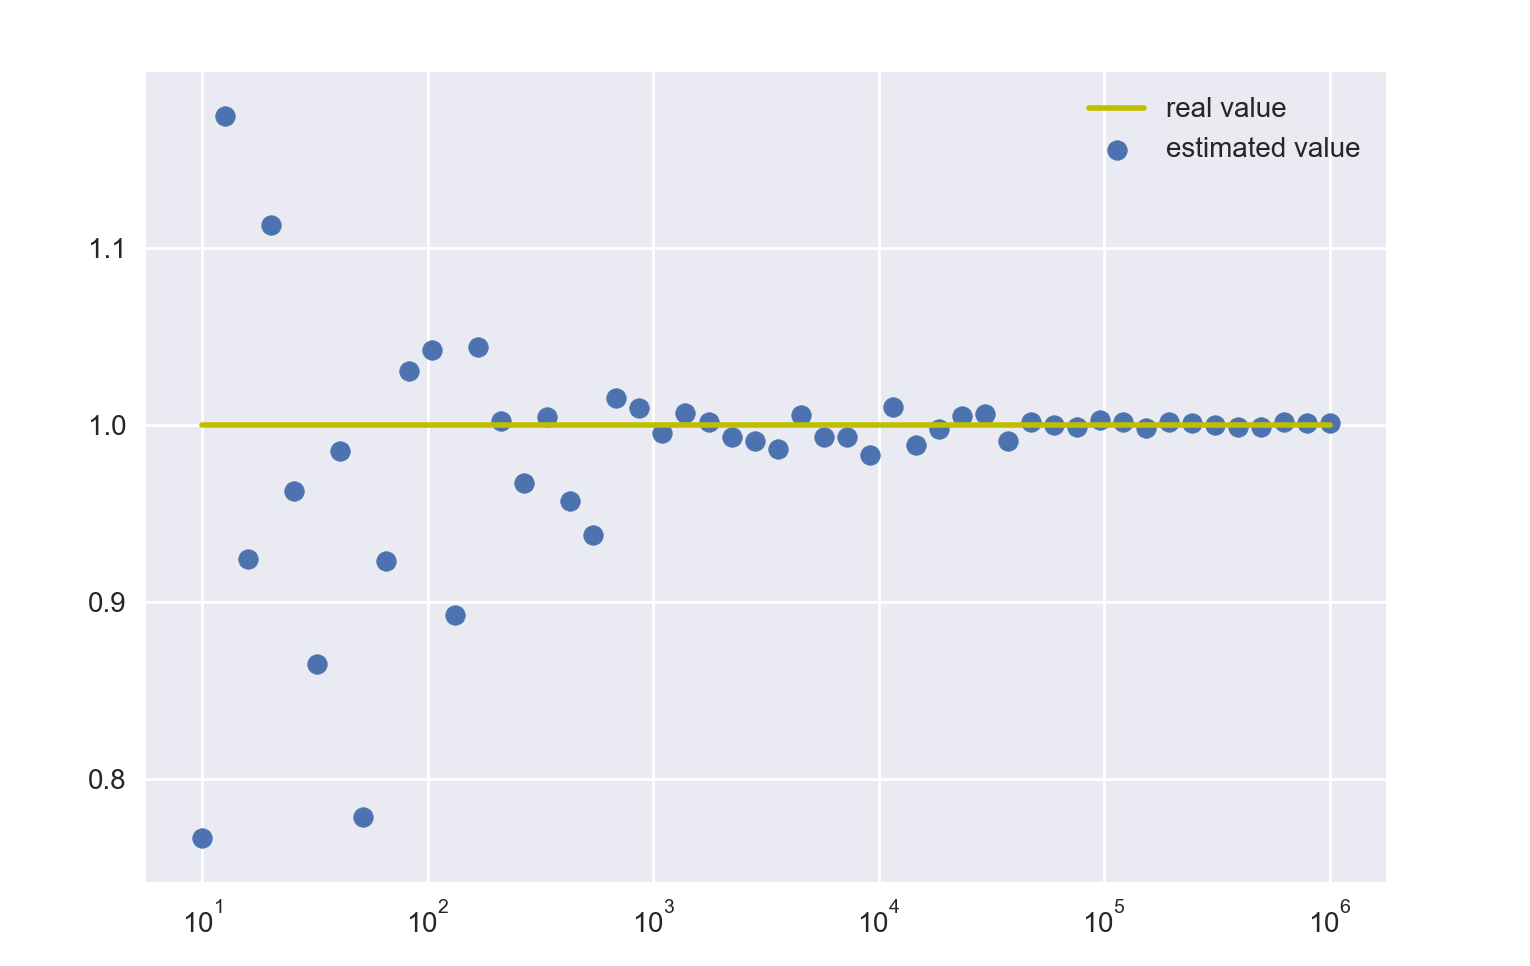
\includegraphics[width=0.8\textwidth]{1}
	\caption{利用MCMC估算$\int_0^1{x e^{x}}$}
\end{figure}

\vspace{1cm}
2)无穷积分计算:\quad $\int_{-\infty}^{\infty}e^{-3x^2}$

通过寻找原函数的方法,求出该积分的值为$\sqrt{\dfrac{\pi}{3}}$。之后利用MCMC方法模拟结果进行比较。由于在计算机中比较容易取得\emph{\textbf{满足正态分布的无穷分布随机数}},这里将g(x)拆分为:
\begin{gather*}
h(x) = \sqrt{2\pi}e^{\frac{-5x^{2}}{2}} \qquad p(x) = \frac{1}{\sqrt{2\pi}} e^{\frac{x^{2}}{2}}
\end{gather*}

之后通过生成一满足服从$-\infty \sim \infty$的随机序列,并将它们通过h(x)进行映射后的结果取平均值,从而得出随机模拟的估计值。

模拟结果如下图。当随机序列元素个数在$10^{5}$个左右时,MCMC估算$\int_{-\infty}^{\infty}e^{-3x^2}$与实际值已十分接近。这说明利用MCMC方法估算积分上下限都为无穷时的无穷积分是有效的。
\begin{figure}[H]
	\centering
	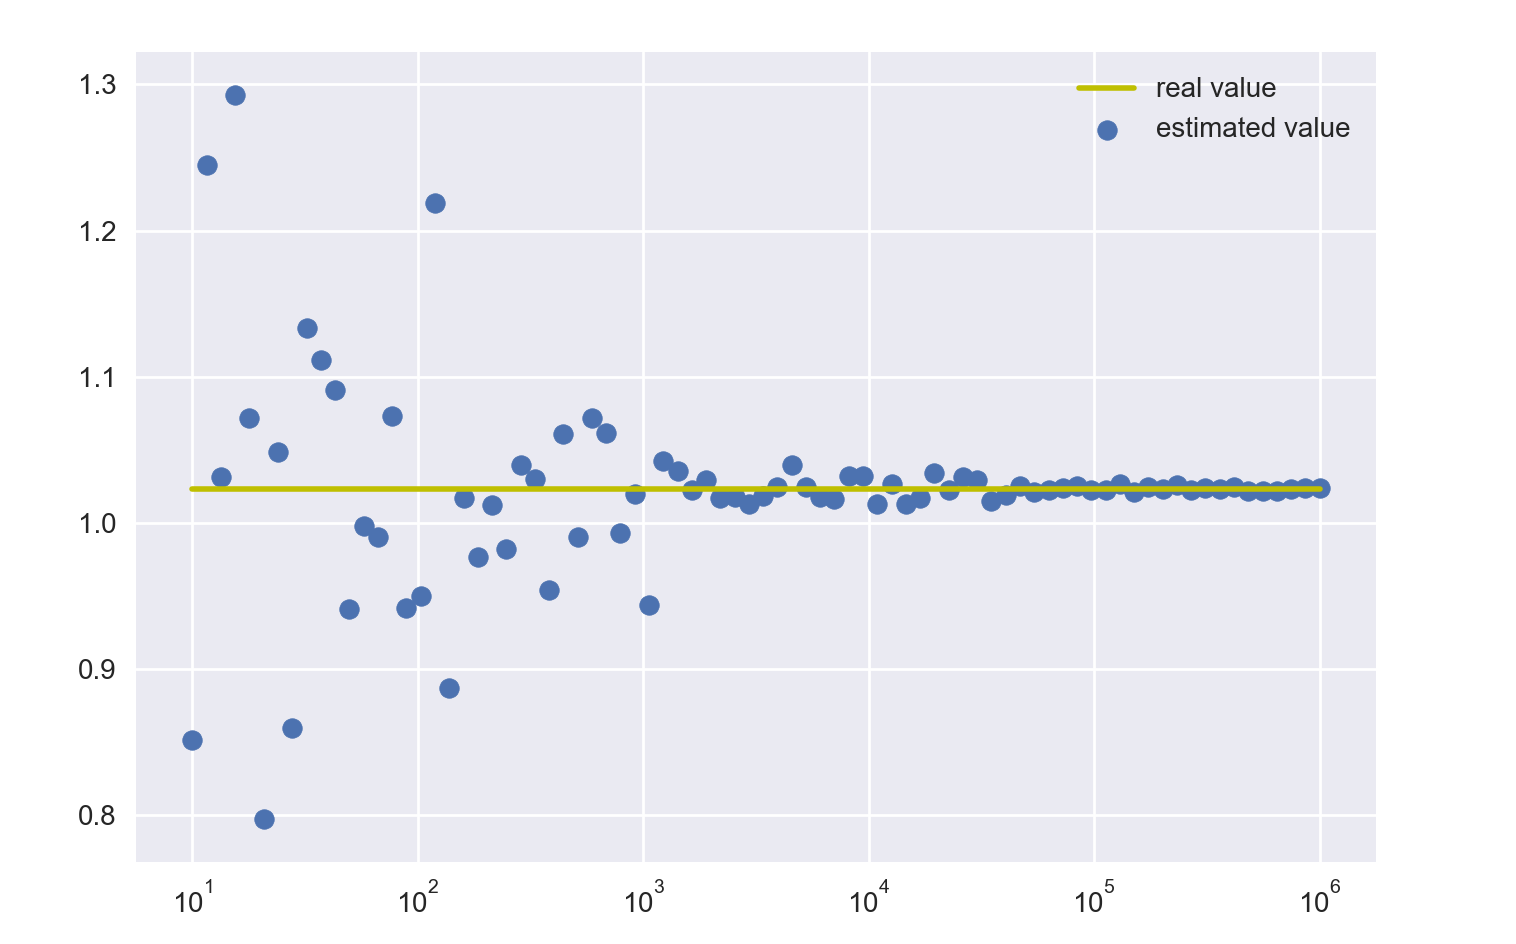
\includegraphics[width = 0.8\textwidth]{quan.png}
	\caption{MCMC估计$\int_{-\infty}^{\infty}e^{-3x^2}$}
\end{figure}

\vspace{1cm}
3)无穷积分计算:\quad $\int_{0}^{\infty}e^{-3x^2}$

通过寻找原函数的方法,求出该积分的值为$\sqrt{\dfrac{\pi}{3}}$。之后利用MCMC方法模拟结果进行比较。由于在计算机中比较容易取得\emph{\textbf{无穷分布的随机数满足正态分布}},这里将g(x)拆分为:
\begin{gather*}
h(x) = \sqrt{2\pi}e^{\frac{-5x^{2}}{2}} \qquad p(x) = \frac{1}{\sqrt{2\pi}} e^{\frac{x^{2}}{2}}
\end{gather*}

之后通过生成一满足服从$0 \sim \infty$的随机序列。由于取值区间为$0 \sim \infty$,故将小于零的随机数映射后的值置为零。即将h(x)设为分段函数:
\begin{equation}
	h(x) = 
	\begin{cases}
		\sqrt{2\pi}e^{\frac{-5x^{2}}{2}} & x \geq 0\\
		0 & otherwise
	\end{cases}
\end{equation}
并将它们通过h(x)进行映射后的结果取平均值,从而得出随机模拟的估计值。由于取值区间在

模拟结果如下。当随机序列元素个数在$10^{4}$个左右时,MCMC估算$\int_{-\infty}^{\infty}e^{-3x^2}$与实际值已十分接近。这说明利用MCMC方法估算积分上下限中有一个为无穷时的无穷积分是有效的。
\begin{figure}[H]
	\centering
	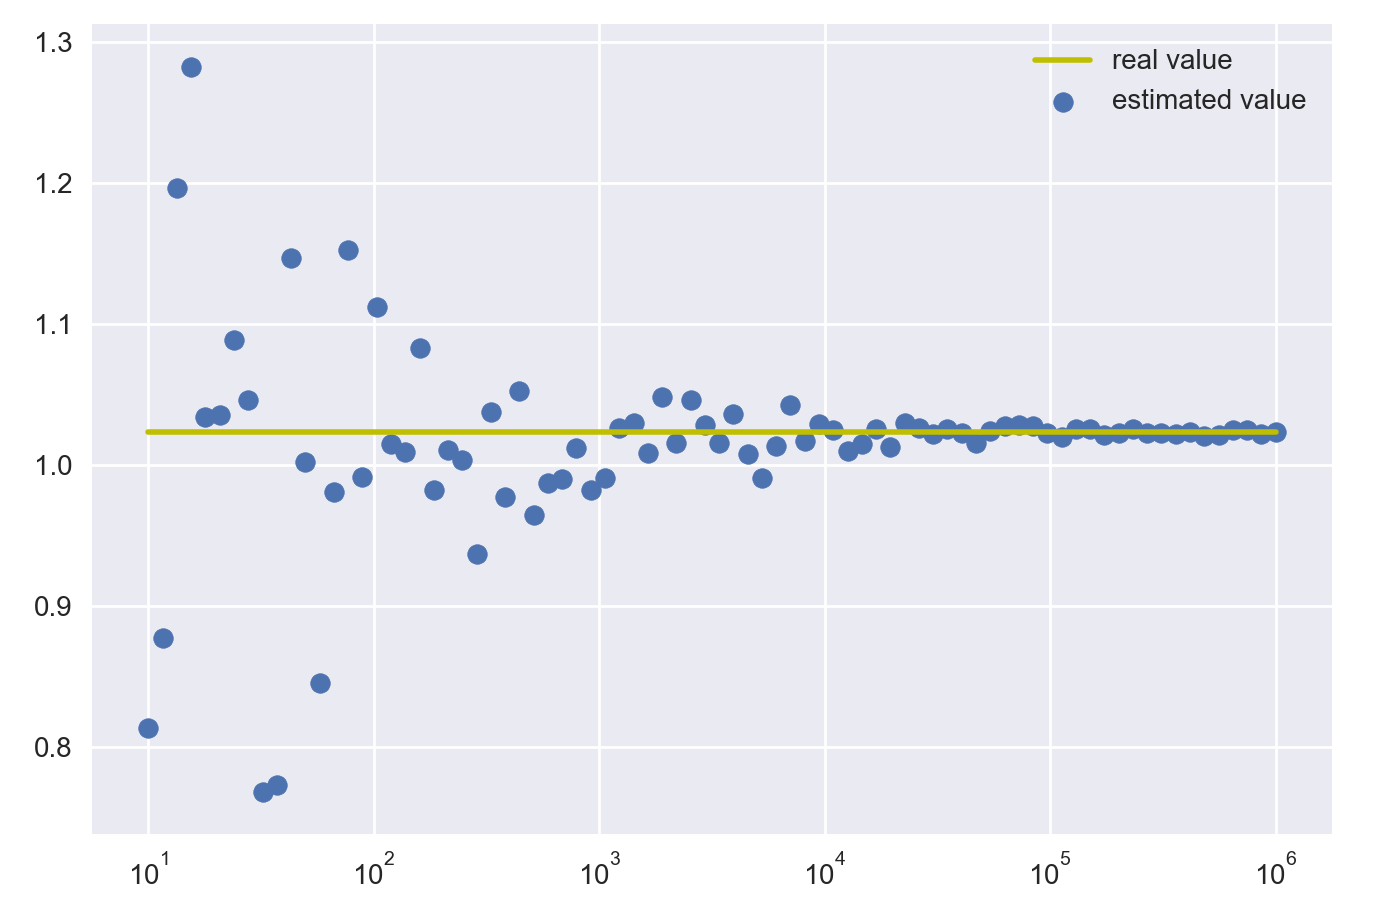
\includegraphics[width = 0.8\textwidth]{ban.png}
	\caption{MCMC估计$\int_{0}^{\infty}e^{-3x^2}$}
\end{figure}

\section{MCMC高维拓展}
当被积函数的维度逐渐增加时,利用传统寻找原函数求积分值的复杂度也大幅上升,而利用MCMC方法模拟估算出积分值则是一种很好的选择。我们可以采用平均期望法来解决这一问题。

假设我们需要解决的高维积分函数为$f(x_{1},x_{2},...,x_{n})$,积分区域为D,我们可以在区域D中随机生成N个点并利用下式进行计算:
\begin{equation}
	\hat{f} = \dfrac{|D|}{N}\sum_{i=1}^{N}f(x_{1}^{(i)},x_{2}^{(i)},...,x_{n}^{(i)})
\end{equation}
其中在这里D为积分区域的体积,在这里$|D| = \prod_{i = 1}^{n}(b_{i}-a_{i})$

\section{平均期望法探究}
接下来我们来探究这种方法的准确性,分别从是否无偏和是否为一致估计量来考虑。为运算简便考虑,这里仅考虑一维情况。

\begin{equation}
\centering
E(\hat{I}) = E(	\frac{b-a}{N}\sum_{i=1}^{N}f(X_{i}) )= \frac{b-a}{N}\sum_{i=1}^{N}E(f(X_{i}) = \int_{a}^{b}f(x) = I
\end{equation}
故这种估算方法采用的是无偏估计量。

之后我们再来研究其是不是一致估计量。
\begin{equation}
	\sigma_{\hat{i}}^{2} = \frac{1}{N}((b-a)\int_{a}^{b}f^{2}(x)-I^2)) = \frac{1}{N}(E(f^{2})-I^{2})\propto N^{-1}
\end{equation}
故这种估算方法采用的是一致估计量。

\section{原函数法与MCMC法对比}
原函数法的优点是计算求得的是真实值,没有误差,但局限在于可求出原函数的积分较少,适用范围小,且计算复杂度高,不易操作。

MCMC方法的优点在与适用性广,不局限于几何形状与问题维数的限制,且容易编程模拟。然而MCMC方法求解的值毕竟是估算,与真实值之间存在着一定误差,且需要大量模拟次数才能得到较为精确的估算值,收敛速度较慢。


\section{附录}
1)定积分计算:   $\int_0^1{x e^{x}}$ 具体代码实现
\pythonexternal{1.py}
\newpage
2)无穷积分计算:\quad $\int_{-\infty}^{\infty}e^{-3x^2}$  具体代码实现
\pythonexternal{2.py}
\vspace{1cm}
3)无穷积分计算:\quad $\int_{0}^{\infty}e^{-3x^2}$ 具体代码实现
\pythonexternal{3.py}


\end{document}